\section{Certified Algorithm}

In this section we initiate the study of certified algorithms for FVS-4CL and the more general 
FVS-BCL. In the final subsection the focus is shifted to the r-Dominating Set problem.



\subsection{FVS-4CL}





In the second stage, we compute a feasible solution $S$, set 
$J_\kappa$\footnote{
    A word on the argument $\kappa$ and the value that we set it to. In our case, for the FVS-4CL problem, 
    $m$ is equal to two. Also, $k = \lceil \frac{2m}{\epsilon} \rceil + 2m \geq 5$. Notice that the set 
    $J_{\kappa}$ is of width $k-2m$, therefore the $m$-neighbourhood (2-neighbourhood) is of width 
    $k - 2m + 2m = k$. Therefore, in our case, the graphs within we stitch are of width
    $k = \lceil \frac{2m}{\epsilon} \rceil + 2m \geq 5$.
    Take for example 
    vertex $v_{2,1}$ in Fig.~\ref{fig:reconfigure}. In order to find every cycle that it is a part of, 
    one would need to consider the layer that it is in, two layers to the left and two layers to the right. 

    \begin{figure}[H]
        \centering
        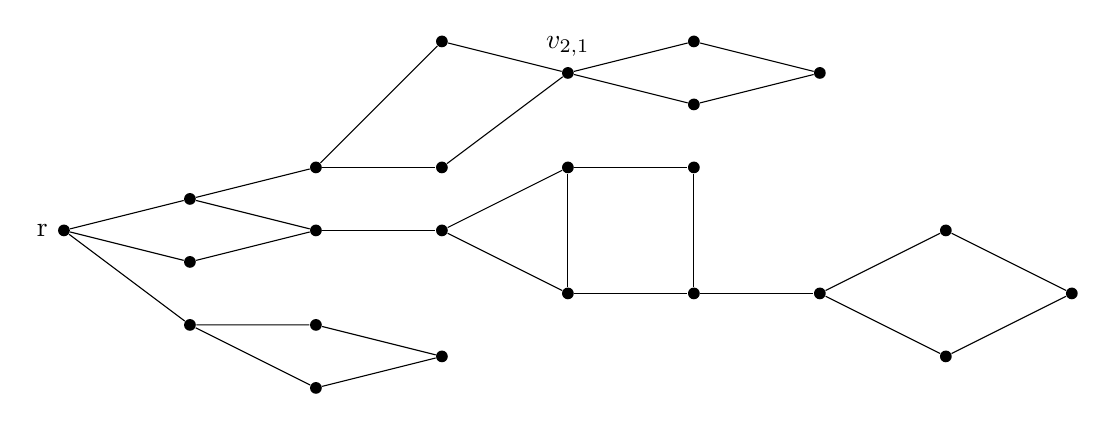
\begin{tikzpicture}[scale=0.8]
    
            \node[fill=black, circle, inner sep=1.5pt, label=left:r] (j02) at (-5,-1) {};
    
            \node[fill=black, circle, inner sep=1.5pt] (j1) at (-3,-2.5) {};
            \node[fill=black, circle, inner sep=1.5pt] (j01) at (-3,-1.5) {};
            \node[fill=black, circle, inner sep=1.5pt] (j03) at (-3,-0.5) {};
    
            \node[fill=black, circle, inner sep=1.5pt] (j04) at (-1,-1) {};
            \node[fill=black, circle, inner sep=1.5pt] (j3) at (-1,0) {};
            \node[fill=black, circle, inner sep=1.5pt] (j4) at (-1,-2.5) {};
            \node[fill=black, circle, inner sep=1.5pt] (n14) at (-1,-3.5) {};
    
    
    
            \node[fill=black, circle, inner sep=1.5pt] (j2) at (1,-1) {};
            \node[fill=black, circle, inner sep=1.5pt] (n12) at (1,2) {};
            \node[fill=black, circle, inner sep=1.5pt] (n13) at (1,0) {};
            \node[fill=black, circle, inner sep=1.5pt] (n15) at (1,-3) {};
    
            \node[fill=black, circle, inner sep=1.5pt] (n11) at (3,0) {};
            \node[fill=black, circle, inner sep=1.5pt] (n16) at (3,-2) {};
    
            \node[fill=black, circle, inner sep=1.5pt, label=above:$v_{2,1}$] (n21) at (3, 1.5) {};
            
            \node[fill=black, circle, inner sep=1.5pt] (n22) at (5,-2) {};
            \node[fill=black, circle, inner sep=1.5pt] (n23) at (5,0) {};
            \node[fill=black, circle, inner sep=1.5pt] (new31) at (5, 2) {};
            \node[fill=black, circle, inner sep=1.5pt] (new32) at (5, 1) {};
    
            \node[fill=black, circle, inner sep=1.5pt] (n32) at (7, -2) {};
            \node[fill=black, circle, inner sep=1.5pt] (new33) at (7,1.5) {};
    
    
            \node[fill=black, circle, inner sep=1.5pt] (n31) at (9, -3) {};
            \node[fill=black, circle, inner sep=1.5pt] (n33) at (9, -1) {};
    
    
            \node[fill=black, circle, inner sep=1.5pt] (n34) at (11, -2) {};
    
            % Draw edges inside J (induced subgraph)
            \draw (j01) -- (j02);
            \draw (j02) -- (j03);
            \draw (j03) -- (j04);
            \draw (j04) -- (j01);
    
            \draw (j4) -- (j1);
    
            \draw (j02) -- (j1);
            \draw (j04) -- (j2);
            \draw (j03) -- (j3);
            
            % Draw edges from J to N^1[J]
            \draw (j2) -- (n11);
            \draw (j2) -- (n16);
            \draw (j3) -- (n12);
            \draw (j1) -- (n14);
            \draw (j3) -- (n13);
            \draw (j4) -- (n15);
    
            % Draw edges inside N^1[J]
            \draw (n14) -- (n15);
            \draw (n16) -- (n11);
    
            % Draw edges between N^1[J] and N^2[J]
            \draw (n16) -- (n22);
            \draw (n11) -- (n23);
            \draw (n13) -- (n21);
            \draw (n12) -- (n21);
    
            % Draw edges between N^2[J] and N^2[J]
            \draw (n22) -- (n23);
    
            % Draw edges between N^2[J] and the other part of the graph
            \draw (n22) -- (n32);
    
            % Draw edges between the edges that are outside of N^2[J]
            \draw (n31) -- (n32);
            \draw (n32) -- (n33);
            \draw (n33) -- (n34);
            \draw (n34) -- (n31);
    
            \draw (n21) -- (new31);
            \draw (n21) -- (new32);
            \draw (new31) -- (new33);
            \draw (new32) -- (new33);
    
    
        \end{tikzpicture}
        \caption{Layer decomposition of graph in Fig.~\ref{fig:first-figure}}
        \label{fig:reconfigure}
    \end{figure}
}

\subsection{FVS-BCL}


\subsection{r-Dominating Set}